\documentclass[tikz, border=5pt]{standalone}

\begin{document}
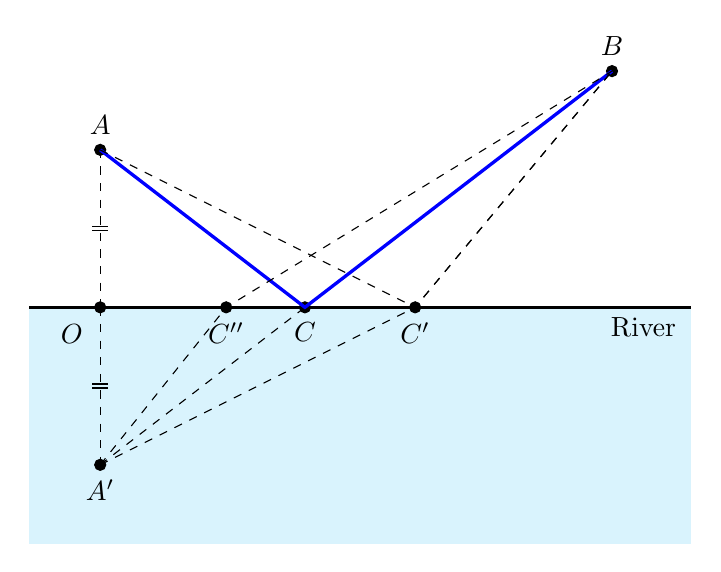
\begin{tikzpicture}

  %% Heron's problem

  % River
  \fill[cyan!15] (0.6,0) rectangle (9,-3);
  \draw[very thick] (0.6,0) -- (9,0);
  \node at (9-0.6,0) [below] {River};

  % Point A
  \draw[fill=black] (1.5,2) circle (2pt);
  \node at (1.5,2) [above=2pt] {\( A \)};

  % Point B
  \draw[fill=black] (8,3) circle (2pt);
  \node at (8,3) [above=2pt] {\( B \)};

  % Point O
  \draw[fill=black] (1.5,0) circle (2pt);
  \node at (1.5,0) [below left=2.8pt] {\( O \)};

  % Line AOA'
  \draw[dashed] (1.5,2) -- (1.5,0);
  \draw[dashed] (1.5,0) -- (1.5,-2);

  % Mark AO and OA' as equal
  \draw[line width=0.5pt] (1.4,0.975) -- (1.6,0.975);
  \draw[line width=0.5pt] (1.4,1.025) -- (1.6,1.025);
  \draw[line width=0.5pt] (1.4,-0.975) -- (1.6,-0.975);
  \draw[line width=0.5pt] (1.4,-1.025) -- (1.6,-1.025);

  % Point A'
  \draw[fill=black] (1.5,-2) circle (2pt);
  \node at (1.5,-2) [below=2pt] {\( A' \)};

  % Path A'B
  \draw[dashed] (1.5,-2) -- (8,3);

  % Intersection point C
  \draw[fill=black] (4.1,0) circle (2pt);
  \node at (4.1,0) [below=2pt] {\( C \)};

  % Path ACB
  \draw[very thick, blue] (1.5,2) -- (4.1,0) -- (8,3);

  % Point C'
  \draw[fill=black] (5.5,0) circle (2pt);
  \node at (5.5,0) [below=2pt] {\( C' \)};

  % Path A'C'B
  \draw[dashed] (1.5,-2) -- (5.5,0) -- (8,3);

  % Path AC'B
  \draw[dashed] (1.5,2) -- (5.5,0) -- (8,3);

  % Point C''
  \draw[fill=black] (3.1,0) circle (2pt);
  \node at (3.1,0) [below=2pt] {\( C'' \)};

  % Path A'C''B
  \draw[dashed] (1.5,-2) -- (3.1,0) -- (8,3);

\end{tikzpicture}
\end{document}
